\documentclass[12pt,a4paper]{report}

% ---------- Geometry ----------
\usepackage[a4paper,left=4cm,right=2.5cm,top=2.5cm,bottom=2.5cm]{geometry}

% ---------- Fonts & Encoding ----------
\usepackage[T1]{fontenc}
\usepackage[utf8]{inputenc}
\usepackage{mathptmx}

% ---------- Core Packages ----------
\usepackage{amsmath}
\usepackage{amssymb}
\usepackage[table]{xcolor}
\usepackage{colortbl}
\usepackage{booktabs}
\usepackage{array}
\usepackage{tabularx}
\usepackage{longtable}
\usepackage{enumitem}
\usepackage{setspace}
\usepackage{titlesec}
\usepackage{fancyhdr}
\usepackage{graphicx}
\usepackage{tikz}
\usetikzlibrary{positioning,calc,shapes.geometric,backgrounds}
\usepackage[skins,breakable]{tcolorbox}
\usepackage{fontawesome5}
\usepackage{listings}
\usepackage[font=small,labelfont={bf,color=ummaroon}]{caption}
\usepackage[hidelinks,colorlinks=false]{hyperref}

% ---------- Colour Palette ----------
\definecolor{ummaroon}{RGB}{115,20,38}
\definecolor{umgold}{RGB}{190,142,25}
\definecolor{umslate}{RGB}{42,52,65}
\definecolor{umoffwhite}{RGB}{250,247,241}

% ---------- Listings style ----------
\lstdefinestyle{umcode}{
  basicstyle=\ttfamily\small,
  keywordstyle=\color{ummaroon}\bfseries,
  commentstyle=\color{umslate!60}\itshape,
  stringstyle=\color{umgold!70!black},
  numbers=left,
  numberstyle=\tiny\color{umslate!50},
  numbersep=8pt,
  frame=single,
  rulecolor=\color{umslate!30},
  backgroundcolor=\color{umoffwhite},
  breaklines=true,
  showstringspaces=false,
  xleftmargin=1.5em
}
\lstset{style=umcode}

% ---------- Chapter / Section styling ----------
\titleformat{\chapter}[display]
  {\normalfont}
  {\textcolor{umgold}{\Large\textsc{Chapter \thechapter}}}
  {8pt}
  {\huge\bfseries\color{umslate}}
  [\vspace{4pt}{\color{umgold}\titlerule[1.4pt]}\vspace{6pt}]
\titlespacing*{\chapter}{0pt}{0pt}{28pt}

\titleformat{\section}
  {\normalfont\Large\bfseries\color{ummaroon}}
  {\thesection}{10pt}{}
\titleformat{\subsection}
  {\normalfont\large\bfseries\color{umslate}}
  {\thesubsection}{8pt}{}

% ---------- Headers / Footers ----------
\setlength{\headheight}{25pt}
\addtolength{\topmargin}{-13pt}
\pagestyle{fancy}
\fancyhf{}
\renewcommand{\headrulewidth}{0.5pt}
\renewcommand{\headrule}{\hbox to\headwidth{\color{umgold}\leaders\hrule height \headrulewidth\hfill}}
\fancyhead[L]{\small\itshape\color{umslate}\leftmark}
\fancyhead[R]{\small\color{umslate}\thepage}
\fancypagestyle{plain}{
  \fancyhf{}
  \fancyfoot[C]{\small\color{umslate}\thepage}
  \renewcommand{\headrulewidth}{0pt}
}

% ---------- Misc ----------
\onehalfspacing
\setlength{\parskip}{4pt}
\setcounter{tocdepth}{2}
\setcounter{secnumdepth}{3}

\newcommand{\highlightbox}[2]{%
  \begin{tcolorbox}[
    enhanced,
    colback=umoffwhite,
    colframe=umslate,
    boxrule=0.6pt,
    left=10pt,right=10pt,top=8pt,bottom=8pt,
    title={\faLightbulb\ #1},
    coltitle=white,
    colbacktitle=ummaroon,
    fonttitle=\bfseries\small,
    attach boxed title to top left={xshift=8pt,yshift=-2pt},
    boxed title style={boxrule=0pt,colframe=ummaroon}
  ]
  #2
  \end{tcolorbox}
}

\begin{document}

% =====================================================
% TITLE PAGE
% =====================================================
\begin{titlepage}
\thispagestyle{empty}
\begin{tikzpicture}[remember picture,overlay]
  \draw[umgold,line width=1.4pt] ($(current page.north west)+(2.2cm,-2.2cm)$) -- ++(1.4cm,0);
  \draw[umgold,line width=1.4pt] ($(current page.north west)+(2.2cm,-2.2cm)$) -- ++(0,-1.4cm);
  \draw[umgold,line width=1.4pt] ($(current page.south east)+(-2.2cm,2.2cm)$) -- ++(-1.4cm,0);
  \draw[umgold,line width=1.4pt] ($(current page.south east)+(-2.2cm,2.2cm)$) -- ++(0,1.4cm);
\end{tikzpicture}

\begin{center}
\vspace*{0.6cm}
{\Large\scshape\color{umslate} University of Malaya}\\[2pt]
{\normalsize\color{umslate!70} Kuala Lumpur, Malaysia}\\[10pt]
{\color{umgold}\rule{5cm}{1pt}}\\[10pt]
{\small\color{umslate} Faculty of Computer Science and Information Technology}

\vspace{2.2cm}
{\Large\bfseries\color{ummaroon}
OPTIMIZING ENERGY CONSUMPTION IN\\[4pt]
DISTRIBUTED IoT SENSOR NETWORKS\\[4pt]
USING ADAPTIVE MACHINE LEARNING\\[4pt]
SCHEDULING
}

\vspace{2.4cm}
{\large\color{umslate} AMIRAH BINTI ZULKIFLI}

\vspace{1.6cm}
{\normalsize\color{umslate}
FACULTY OF COMPUTER SCIENCE AND INFORMATION TECHNOLOGY\\
UNIVERSITY OF MALAYA\\
KUALA LUMPUR
}

\vspace{1.4cm}
{\normalsize\color{umslate} 2026}

\end{center}

\vfill
\begin{center}
\footnotesize\color{umslate!70}
\textit{Unofficial template --- not affiliated with or endorsed by the university.\\
Sample content only.}
\end{center}
\vspace{0.4cm}
\end{titlepage}

% =====================================================
% SECOND TITLE PAGE (with degree statement)
% =====================================================
\newpage
\thispagestyle{empty}
\begin{center}
\vspace*{0.6cm}
{\Large\bfseries\color{ummaroon}
OPTIMIZING ENERGY CONSUMPTION IN\\[4pt]
DISTRIBUTED IoT SENSOR NETWORKS\\[4pt]
USING ADAPTIVE MACHINE LEARNING\\[4pt]
SCHEDULING
}

\vspace{2.0cm}
{\large\color{umslate} AMIRAH BINTI ZULKIFLI}

\vspace{2.0cm}
{\normalsize\color{umslate}
\parbox{11cm}{\centering
THESIS SUBMITTED IN FULFILMENT OF THE REQUIREMENTS\\
FOR THE DEGREE OF MASTER OF COMPUTER SCIENCE
}}

\vspace{2.0cm}
{\normalsize\color{umslate}
FACULTY OF COMPUTER SCIENCE AND INFORMATION TECHNOLOGY\\
UNIVERSITY OF MALAYA\\
KUALA LUMPUR
}

\vspace{1.4cm}
{\normalsize\color{umslate} 2026}
\end{center}

\vfill
\begin{center}
\footnotesize\color{umslate!70}
\textit{Unofficial template --- not affiliated with or endorsed by the university.\\
Sample content only. All names, data and findings herein are fictional.}
\end{center}

% =====================================================
% FRONT MATTER
% =====================================================
\pagenumbering{roman}

\chapter*{Original Literary Work Declaration}
\addcontentsline{toc}{chapter}{Original Literary Work Declaration}

\noindent Name of Candidate: \textbf{Amirah binti Zulkifli} \hfill Matric No.: \textbf{WGA 21 0001}

\medskip
\noindent Name of Degree: \textbf{Master of Computer Science}

\medskip
\noindent Title of Thesis (``this Work''):

\begin{quote}
\itshape Optimizing Energy Consumption in Distributed IoT Sensor Networks Using Adaptive Machine Learning Scheduling
\end{quote}

\noindent Field of Study: \textbf{Distributed Systems and Machine Learning}

\bigskip
\noindent I do solemnly and sincerely declare that:
\begin{enumerate}[label=(\arabic*)]
  \item I am the sole author/writer of this Work;
  \item This Work is original;
  \item Any use of any work in which copyright exists was done by way of fair dealing and for permitted purposes and any excerpt or extract from, or reference to or reproduction of any copyright work has been disclosed expressly and sufficiently and the title of the Work and its authorship have been acknowledged in this Work;
  \item I do not have any actual knowledge nor do I ought reasonably to know that the making of this Work constitutes an infringement of any copyright work;
  \item I hereby assign all and every rights in the copyright to this Work to the University of Malaya (``UM''), who henceforth shall be owner of the copyright in this Work and that any reproduction or use in any form or by any means whatsoever is prohibited without the written consent of UM having been first had and obtained;
  \item I am fully aware that if in the course of making this Work I have infringed any copyright whether intentionally or otherwise, I may be subject to legal action or any other action as may be determined by UM.
\end{enumerate}

\vspace{1.4cm}
\noindent Candidate's Signature \hfill Date

\vspace{1.0cm}
\noindent Subscribed and solemnly declared before,

\vspace{1.4cm}
\noindent Witness's Signature \hfill Date

\medskip
\noindent Name: \textit{Prof. Dr. Nurul Huda binti Ismail}\\
Designation: \textit{Supervisor}

\bigskip
\begin{center}
\footnotesize\color{umslate!70}\textit{Sample declaration text for template demonstration only.}
\end{center}

% ---------- Abstrak ----------
\chapter*{Abstrak}
\addcontentsline{toc}{chapter}{Abstrak}

Rangkaian penderia Internet Pelbagai Benda (IoT) yang diagihkan sering beroperasi di bawah kekangan
tenaga yang ketat, terutamanya dalam penempatan bangunan pintar berskala besar. Kajian ini
mencadangkan rangka kerja penjadualan adaptif berasaskan pembelajaran mesin yang menyesuaikan
kadar persampelan penderia secara dinamik berdasarkan corak beban rangkaian dan variasi persekitaran.
Rangka kerja ini dinilai menggunakan set data dunia sebenar yang dikumpul daripada penempatan
bangunan pintar Nexa Systems di Kuala Lumpur, merangkumi 48 penderia sepanjang tempoh 90 hari.
Keputusan eksperimen menunjukkan pengurangan penggunaan tenaga sebanyak 27.4\% berbanding
penjadualan kadar tetap konvensional, dengan peningkatan kependaman data purata yang boleh diabaikan
(kurang daripada 120 milisaat). Sumbangan utama kajian ini ialah algoritma penjadualan ringan yang
sesuai untuk penggunaan pada get pinggir (edge gateway) dengan sumber terhad, serta metodologi
penilaian yang boleh disesuaikan untuk topologi rangkaian penderia yang lain.

\medskip
\noindent\textbf{Kata kunci:} Internet Pelbagai Benda, pembelajaran mesin, kecekapan tenaga,
pengkomputeran pinggir, penjadualan adaptif

% ---------- Abstract ----------
\chapter*{Abstract}
\addcontentsline{toc}{chapter}{Abstract}

Distributed Internet of Things (IoT) sensor networks frequently operate under tight energy
constraints, particularly in large-scale smart building deployments. This thesis proposes an
adaptive, machine-learning-based scheduling framework that dynamically adjusts sensor sampling
rates in response to network load patterns and ambient environmental variance. The framework is
evaluated on a real-world dataset collected from a Nexa Systems smart building deployment in
Kuala Lumpur, comprising 48 sensors over a 90-day observation window. Experimental results show a
27.4\% reduction in aggregate energy consumption compared to conventional fixed-rate scheduling,
with a negligible increase in average data latency (under 120 milliseconds). The key contributions
of this work are: (i) a lightweight scheduling algorithm suitable for deployment on
resource-constrained edge gateways, and (ii) a reusable evaluation methodology applicable to other
sensor network topologies.

\medskip
\noindent\textbf{Keywords:} Internet of Things, machine learning, energy efficiency, edge
computing, adaptive scheduling

% ---------- Acknowledgements ----------
\chapter*{Acknowledgements}
\addcontentsline{toc}{chapter}{Acknowledgements}

I would like to express my deepest gratitude to my supervisor, Prof. Dr. Nurul Huda binti Ismail,
for her invaluable guidance, patience, and constructive feedback throughout the course of this
research. Her insistence on methodological rigour shaped every chapter of this thesis.

I am also thankful to the Faculty of Computer Science and Information Technology, University of
Malaya, for providing the computing resources and laboratory space that made this work possible.
My appreciation extends to the engineering team at Nexa Systems for granting access to their smart
building sensor infrastructure and for their technical support during data collection.

Finally, I wish to thank my family and fellow postgraduate colleagues in the Distributed Systems
Research Group for their encouragement, and the anonymous reviewers whose comments substantially
improved the clarity of this work.

% ---------- TOC / LOF / LOT ----------
\tableofcontents
\clearpage
\listoffigures
\addcontentsline{toc}{chapter}{List of Figures}
\clearpage
\listoftables
\addcontentsline{toc}{chapter}{List of Tables}

\chapter*{List of Symbols and Abbreviations}
\addcontentsline{toc}{chapter}{List of Symbols and Abbreviations}
\begin{description}[leftmargin=2.6cm,style=nextline]
  \item[IoT] Internet of Things
  \item[ML] Machine Learning
  \item[MAE] Mean Absolute Error
  \item[RMSE] Root Mean Square Error
  \item[$\lambda$] Adaptive sampling rate coefficient
  \item[$\Delta E$] Change in aggregate energy consumption
  \item[QoS] Quality of Service
  \item[LSTM] Long Short-Term Memory (recurrent neural network)
\end{description}

% =====================================================
% MAIN MATTER
% =====================================================
\clearpage
\pagenumbering{arabic}

\chapter{Introduction}
\label{ch:intro}

\section{Background of Study}

The proliferation of Internet of Things (IoT) sensor networks in smart building management has
created a pressing need for energy-aware operational strategies. A typical mid-sized commercial
building deployment may involve dozens of battery-powered or energy-harvesting sensor nodes
continuously reporting temperature, humidity, occupancy, and air-quality readings to a central
analytics platform. When these nodes sample and transmit data at fixed intervals regardless of
actual environmental variability or network conditions, substantial energy is wasted on redundant
or low-value transmissions.

Nexa Systems, a facilities-technology provider operating several smart building pilots in Kuala
Lumpur, reported that fixed-rate sensor polling accounted for approximately 34\% of total edge
device energy draw across their 2025 deployment portfolio. This observation motivates the central
question of this thesis: can a machine-learning-driven scheduler reduce energy consumption
without materially degrading the timeliness of environmental data delivered to downstream
analytics services?

\section{Problem Statement}

Existing sensor scheduling approaches fall broadly into two categories. Fixed-rate schedulers are
simple to implement but cannot adapt to changing conditions, leading to energy waste during
periods of environmental stability. Threshold-based adaptive schedulers respond to sensed changes
but typically rely on hand-tuned heuristics that generalise poorly across building types and
climates. Neither approach jointly optimises for energy consumption and data latency in a
principled, data-driven manner, and few published evaluations use sustained real-world deployment
data rather than simulated traces.

\section{Research Objectives}

This study pursues three objectives:
\begin{enumerate}[label=RO\arabic*.]
  \item To design an adaptive scheduling framework that predicts appropriate sensor sampling
        intervals using historical network load and environmental variance.
  \item To implement the framework as a lightweight component deployable on resource-constrained
        edge gateways.
  \item To empirically evaluate the framework's energy and latency trade-offs against fixed-rate
        and threshold-based baselines using a real-world smart building dataset.
\end{enumerate}

\section{Research Questions}

\begin{enumerate}[label=RQ\arabic*.]
  \item How much can aggregate energy consumption be reduced through adaptive, machine-learning-based
        sensor scheduling compared to fixed-rate scheduling?
  \item What is the resulting impact on end-to-end data latency and downstream analytics accuracy?
  \item Which environmental and network-load features contribute most strongly to scheduling
        decisions?
\end{enumerate}

\highlightbox{Research Highlights}{
\begin{itemize}[leftmargin=1.4em,itemsep=2pt]
  \item[\faBolt] 27.4\% aggregate energy reduction over fixed-rate scheduling.
  \item[\faClock] Median latency overhead below 120\,ms.
  \item[\faDatabase] Evaluated on a 90-day, 48-sensor real-world deployment dataset.
  \item[\faMicrochip] Designed for deployment on constrained edge gateway hardware.
\end{itemize}
}

\section{Scope and Limitations}

The study is scoped to indoor environmental sensing (temperature, humidity, occupancy, and
CO$_2$) in commercial office buildings and does not address outdoor or industrial sensor
networks. The evaluation dataset is drawn from a single facilities partner (Nexa Systems); while
the deployment spans three building zones, results may not generalise to markedly different
climates or building typologies without retraining.

\section{Organisation of the Thesis}

Chapter~\ref{ch:litreview} reviews related work on sensor scheduling and edge-based machine
learning. Chapter~\ref{ch:methodology} presents the proposed methodology, dataset, and evaluation
design. Subsequent chapters (omitted from this template excerpt) would report experimental results
and conclusions.

\chapter{Literature Review}
\label{ch:litreview}

\section{Sensor Scheduling Strategies}

Early work on wireless sensor network longevity focused primarily on duty-cycling: periodically
switching radios and sensing elements into low-power states. While effective for extending battery
life, pure duty-cycling schemes are agnostic to the informational value of each reading, and may
either oversample stable environments or undersample rapidly changing ones.

Threshold-based adaptive schemes improve on this by triggering additional samples when a sensed
value crosses a predefined delta, but the thresholds are usually static and tuned per deployment,
requiring manual recalibration when building occupancy patterns change.

\section{Machine Learning for Edge Scheduling}

More recent studies have explored using lightweight predictive models -- decision trees, gradient
boosted ensembles, and compact recurrent networks -- to forecast short-term environmental
variability and adjust sampling intervals accordingly. These approaches generally report energy
savings in the range of 15--30\% over fixed-rate baselines, though comparability across studies is
limited by inconsistent evaluation datasets and metrics.

Table~\ref{tab:related-work} summarises representative approaches from the reviewed literature.

\begin{table}[htbp]
\centering
\caption{Summary of related scheduling approaches}
\label{tab:related-work}
\begin{tabularx}{\textwidth}{@{}p{2.6cm}p{3.0cm}p{3.6cm}X@{}}
\toprule
\rowcolor{ummaroon!85}
\textcolor{white}{\textbf{Approach}} & \textcolor{white}{\textbf{Adaptivity}} &
\textcolor{white}{\textbf{Evaluation Data}} & \textcolor{white}{\textbf{Reported Limitation}} \\
\midrule
Fixed-rate duty cycling & None & Simulated traces & Ignores informational value of readings \\
\addlinespace
Threshold-based adaptive & Rule-based & Small pilot deployments & Manual per-site threshold tuning \\
\addlinespace
Regression-based forecasting & Statistical & Single-building datasets & Limited cross-building generalisation \\
\addlinespace
LSTM-based scheduling & Learned, sequential & Synthetic + short pilots & High inference cost on constrained gateways \\
\bottomrule
\end{tabularx}
\end{table}

\section{Research Gap}

Across the reviewed literature, three gaps recur: (i) limited use of sustained, multi-month
real-world deployment data; (ii) insufficient attention to inference cost on constrained edge
hardware; and (iii) a lack of joint optimisation for both energy and latency objectives. This
thesis addresses all three by evaluating a lightweight, gateway-deployable scheduler on a 90-day
real-world dataset with explicit energy--latency trade-off analysis.

\section{Conceptual Framework}

Figure~\ref{fig:framework} illustrates the conceptual framework guiding this study. Network load
and environmental variance jointly inform the adaptive scheduling algorithm, whose output --
sensor sampling interval -- determines the resulting energy consumption and data latency.

\begin{figure}[htbp]
\centering
\begin{tikzpicture}[
  node distance=1.0cm and 1.6cm,
  box/.style={draw=umslate,thick,rounded corners=3pt,fill=umoffwhite,
              align=center,minimum width=3.1cm,minimum height=1.05cm,font=\small},
  outbox/.style={draw=ummaroon,thick,rounded corners=3pt,fill=ummaroon!8,
              align=center,minimum width=3.1cm,minimum height=1.05cm,font=\small}
]
  \node[box] (iv1) {Sensor Sampling\\Rate History};
  \node[box, below=of iv1] (iv2) {Network Load\\Pattern};
  \node[box, below=of iv2] (iv3) {Ambient\\Variance};

  \node[box, right=2.2cm of iv2, minimum height=2.4cm] (process) {Adaptive\\Scheduling\\Algorithm};

  \node[outbox, right=2.2cm of process, above=0.35cm of process.east, anchor=west] (dv1) {Energy\\Consumption};
  \node[outbox, right=2.2cm of process, below=0.35cm of process.east, anchor=west] (dv2) {Data\\Latency};

  \draw[->,thick,umslate] (iv1) -- (process.150);
  \draw[->,thick,umslate] (iv2) -- (process.west);
  \draw[->,thick,umslate] (iv3) -- (process.210);
  \draw[->,thick,ummaroon] (process.20) -- (dv1.west);
  \draw[->,thick,ummaroon] (process.-20) -- (dv2.west);
\end{tikzpicture}
\caption{Conceptual framework linking scheduling inputs to energy and latency outcomes}
\label{fig:framework}
\end{figure}

\chapter{Methodology}
\label{ch:methodology}

\section{Research Design}

This study follows a design-science research approach: an artefact (the adaptive scheduler) is
designed, implemented, and evaluated against baseline artefacts using quantitative metrics derived
from a real-world dataset. The methodology comprises four phases: data collection, feature
engineering, model training, and comparative evaluation.

\section{System Architecture}

Figure~\ref{fig:architecture} depicts the end-to-end system architecture used in this study. Sensor
nodes stream readings to an edge gateway, which hosts the adaptive scheduler and performs local
preprocessing before forwarding aggregated data to a cloud analytics platform.

\begin{figure}[htbp]
\centering
\begin{tikzpicture}[
  node distance=0.5cm and 1.3cm,
  comp/.style={draw=umslate,thick,rounded corners=3pt,fill=umoffwhite,
               align=center,minimum width=2.6cm,minimum height=1.3cm,font=\small}
]
  \node[comp] (sensors) {Sensor Layer\\[1pt]\footnotesize Temp / Humidity / CO$_2$};
  \node[comp, right=of sensors] (gateway) {Edge Gateway\\[1pt]\footnotesize Adaptive Scheduler};
  \node[comp, right=of gateway] (cloud) {Cloud Analytics\\[1pt]\footnotesize Synapse Platform};
  \node[comp, right=of cloud] (dash) {Facilities\\Dashboard};

  \draw[->,thick,umslate] (sensors) -- (gateway);
  \draw[->,thick,umslate] (gateway) -- (cloud);
  \draw[->,thick,umslate] (cloud) -- (dash);

  \begin{scope}[on background layer]
    \draw[fill=umgold!15,draw=none,rounded corners=4pt]
      ($(sensors.north west)+(-0.25cm,0.25cm)$) rectangle ($(gateway.south east)+(0.25cm,-0.25cm)$);
  \end{scope}
\end{tikzpicture}
\caption{System architecture from sensor layer to facilities dashboard}
\label{fig:architecture}
\end{figure}

\section{Dataset}

Data were collected from a Nexa Systems smart building deployment comprising three office zones in
Kuala Lumpur, using 48 sensor nodes over a continuous 90-day period between March and June 2026.
Table~\ref{tab:dataset} summarises the dataset composition.

\begin{table}[htbp]
\centering
\caption{Dataset description}
\label{tab:dataset}
\begin{tabularx}{\textwidth}{@{}Xrr@{}}
\toprule
\rowcolor{umslate}
\textcolor{white}{\textbf{Attribute}} & \textcolor{white}{\textbf{Value}} & \textcolor{white}{\textbf{Unit}} \\
\midrule
Deployment duration & 90 & days \\
Number of sensor nodes & 48 & nodes \\
Building zones & 3 & zones \\
Baseline sampling interval & 30 & seconds \\
Total raw readings collected & 12.4 & million \\
Missing-data rate after cleaning & 1.8 & \% \\
\bottomrule
\end{tabularx}
\end{table}

\section{Feature Engineering}

Three feature groups were derived from the raw sensor stream: (i) rolling statistics of past
readings (mean, variance, rate of change) over 5-, 15-, and 60-minute windows; (ii) network load
indicators, including gateway queue depth and transmission retry count; and (iii) contextual
features such as time-of-day and occupancy state inferred from motion sensors.

\section{Adaptive Scheduling Model}

The scheduler uses a compact gradient-boosted regression model to predict the next appropriate
sampling interval $\Delta t$ for each sensor, subject to a minimum interval $\Delta t_{\min}=10$s
and maximum interval $\Delta t_{\max}=300$s:

\begin{equation}
\Delta t = \mathrm{clip}\left(\lambda \cdot f(\mathbf{x}), \; \Delta t_{\min}, \; \Delta t_{\max}\right)
\label{eq:scheduler}
\end{equation}

\noindent where $f(\mathbf{x})$ is the model's predicted stability score for feature vector
$\mathbf{x}$, and $\lambda$ is a tunable aggressiveness coefficient calibrated on a validation
split. The model was selected for its low inference latency relative to recurrent alternatives,
making it suitable for deployment on constrained edge gateway hardware.

\section{Evaluation Metrics}

Table~\ref{tab:metrics} lists the metrics used to compare the proposed scheduler against fixed-rate
and threshold-based baselines.

\begin{table}[htbp]
\centering
\caption{Evaluation metrics}
\label{tab:metrics}
\begin{tabularx}{\textwidth}{@{}p{3.2cm}X@{}}
\toprule
\rowcolor{ummaroon!85}
\textcolor{white}{\textbf{Metric}} & \textcolor{white}{\textbf{Description}} \\
\midrule
Aggregate energy consumption & Total estimated energy draw across all sensor nodes, in kWh \\
\addlinespace
Data latency & Time between sensor event occurrence and dashboard availability, in ms \\
\addlinespace
MAE / RMSE & Prediction error of downstream analytics trained on scheduled data \\
\addlinespace
Sampling reduction ratio & Proportion decrease in total transmitted readings versus baseline \\
\bottomrule
\end{tabularx}
\end{table}

\section{Experimental Procedure}

Listing~\ref{lst:scheduler} shows a simplified pseudocode excerpt of the scheduling loop executed
on each edge gateway.

\begin{lstlisting}[language=Python,caption={Simplified adaptive scheduling loop},label={lst:scheduler}]
def next_interval(sensor_id, feature_window):
    # f(x): predicted stability score from gradient-boosted model
    stability = model.predict(feature_window)
    interval = LAMBDA * stability
    return clip(interval, MIN_INTERVAL, MAX_INTERVAL)

def scheduling_loop(sensor_id):
    while True:
        window = collect_features(sensor_id)
        dt = next_interval(sensor_id, window)
        sample_and_transmit(sensor_id)
        sleep(dt)
\end{lstlisting}

Each baseline and the proposed scheduler were run over an identical 14-day held-out evaluation
window, with results aggregated per building zone to control for occupancy differences.

\chapter*{References}
\addcontentsline{toc}{chapter}{References}
\begin{thebibliography}{99}

\bibitem{abdullah2024} Abdullah, R., \& Krishnan, S. (2024). Duty-cycled wireless sensor networks
for building automation: A survey. \textit{Journal of Ambient Intelligence and Smart Environments},
16(2), 145--167.

\bibitem{chen2023} Chen, L., Osman, F., \& Hartono, D. (2023). Threshold-adaptive sampling for
indoor environmental monitoring. \textit{Sensors and Actuators Reports}, 5, 100089.

\bibitem{ibrahim2025} Ibrahim, N. A., \& Wong, K. M. (2025). Energy-latency trade-offs in edge
machine learning for IoT scheduling. \textit{IEEE Internet of Things Journal}, 12(4), 3312--3325.

\bibitem{lopez2022} Lopez, M., \& Tan, C. H. (2022). A comparative study of recurrent models for
short-horizon environmental forecasting. In \textit{Proceedings of the International Conference on
Pervasive Computing}, 88--97.

\bibitem{nexa2025} Nexa Systems. (2025). \textit{Smart building energy portfolio report 2025}.
Internal technical report.

\bibitem{rahman2021} Rahman, A. F., \& Zulkifli, S. (2021). Gradient boosted ensembles for
resource-constrained inference: A benchmark study. \textit{Journal of Edge Computing Systems},
3(1), 22--40.

\bibitem{santos2024} Santos, P., \& Yusof, H. (2024). Design-science methodology in applied
computer science research. \textit{Computing Research Methods Quarterly}, 9(3), 201--219.

\bibitem{tanaka2023} Tanaka, Y., \& Rashid, M. (2023). Occupancy-aware sensing for commercial
office buildings. \textit{Building and Environment}, 228, 109876.

\end{thebibliography}

\appendix
\chapter{Sample Feature Definitions}
\label{app:features}

Table~\ref{tab:features} lists a subset of engineered features used to train the adaptive
scheduling model, provided here as a template illustration of an appendix table.

\begin{table}[htbp]
\centering
\caption{Sample engineered features}
\label{tab:features}
\begin{tabularx}{\textwidth}{@{}p{3.4cm}X@{}}
\toprule
\rowcolor{umslate}
\textcolor{white}{\textbf{Feature}} & \textcolor{white}{\textbf{Description}} \\
\midrule
\texttt{roll\_mean\_15m} & Rolling mean of sensor reading over a 15-minute window \\
\addlinespace
\texttt{roll\_var\_60m} & Rolling variance of sensor reading over a 60-minute window \\
\addlinespace
\texttt{queue\_depth} & Current transmission queue depth at the edge gateway \\
\addlinespace
\texttt{occupancy\_flag} & Binary indicator of inferred room occupancy \\
\addlinespace
\texttt{retry\_count\_5m} & Number of transmission retries in the preceding 5 minutes \\
\bottomrule
\end{tabularx}
\end{table}

\chapter{Sample Interview Guide}
\label{app:interview}

The following questions were used in template form during facilities-staff consultation sessions
regarding acceptable latency thresholds for dashboard alerts.

\begin{enumerate}[label=Q\arabic*.]
  \item What is the maximum acceptable delay between a sensor event and its appearance on the
        facilities dashboard for routine monitoring?
  \item Are there specific zones or times of day requiring stricter latency guarantees?
  \item How should the system balance battery replacement frequency against alert responsiveness?
\end{enumerate}

\end{document}
